The choice of the kinematical description of the continuum is 
extremely important for the development of a computational code, 
since it directly affects the accuracy of the numerical result. 
In the literature, two classic descriptions are commonly used, 
namely Lagrangian and Eulerian.

\medskip
The Lagrangian description is one where each computational mesh node (black point) 
moves at the same velocity as the material point (white square), as can be seen in
\ref{ale fig}a. Thus, for each time step, we have a new computational mesh. 
The main advantage of this description is that the value of the 
computational mesh node will have the same value as the material point
 and thus, numerical diffusion will not be observed. In addition, 
the Lagrangian description makes it possible to perform 
fluid-structure interaction simulations. However, for large 
deformations, it is necessary to implement an insetion and deletion
node algorithm for computational mesh.

\medskip
The Eulerian description is the one where the computational mesh node 
remains fixed for each time step, as can be seen in \ref{ale fig}b.
Thus, the computational mesh node value will be an interpolation 
of the material point, causing the presence of numerical diffusion 
in the solution. However, the computational cost is relatively 
attractive since it is not necessary the remeshing in each time step.

\medskip
A description, however, that combines the advantages of these two 
classic descriptions as well as minimizing their disadvantages would be
most appropriate. In this context that the Arbitrary 
Lagrangian-Eulerian description (ALE) was developed. 
This description considers that the velocity field of computational 
mesh is unlike than the material point and null value, as can be seen 
in \ref{ale fig}c. In this way, it can be calculated as a 
linear combination of other velocity fields, so that we have an 
optimal relationship between numerical diffusion and mesh deformation. 
In addition, it is possible to assign several velocity values to 
specific regions of the problem in order to improve the 
accuracy of the solution.



\begin{figure}[H]
\caption{One-dimensional examples of the classical descriptions}
\begin{center}
\begin{tikzpicture}[scale=1.7]

 % (a) Lagrangian
 % -------------------------------------------------------------------
 % bottom line
 \draw[line width=0pt] (0,5) -- (6,5);


 % mesh motion
 \draw [line width=0pt] (0,  5) -- (0.5,6)  ;
 \draw [line width=0pt] (1,  5) -- (1.4,6)  ;
 \draw [line width=0pt] (2.7,5) -- (2.3,6);
 \draw [line width=0pt] (4,  5) -- (3.5,6)  ;
 \draw [line width=0pt] (5.1,5) -- (4.6,6);
 \draw [line width=0pt] (6,  5) -- (5.4,6)  ;

 % particle motion
 \draw [dashed,line width=0pt] (0,  5) -- (0.5,6)  ; 
 \draw [dashed,line width=0pt] (1,  5) -- (1.4,6)  ; 
 \draw [dashed,line width=0pt] (2.7,5) -- (2.3,6);   
 \draw [dashed,line width=0pt] (4,  5) -- (3.5,6)  ; 
 \draw [dashed,line width=0pt] (5.1,5) -- (4.6,6);   
 \draw [dashed,line width=0pt] (6,  5) -- (5.4,6)  ; 



 \node[square, fill=white, draw, inner sep=0pt, minimum size=9pt] at (0,5) {};
 \node[square, fill=white, draw, inner sep=0pt, minimum size=9pt] at (1,5) {};
 \node[square, fill=white, draw, inner sep=0pt, minimum size=9pt] at (2.7,5) {};
 \node[square, fill=white, draw, inner sep=0pt, minimum size=9pt] at (4,5) {};
 \node[square, fill=white, draw, inner sep=0pt, minimum size=9pt] at (5.1,5) {};
 \node[square, fill=white, draw, inner sep=0pt, minimum size=9pt] at (6,5) {};

 \node[circle, fill=black, inner sep=0pt, minimum size=5pt] at (0,5) {};
 \node[circle, fill=black, inner sep=0pt, minimum size=5pt] at (1,5) {};
 \node[circle, fill=black, inner sep=0pt, minimum size=5pt] at (2.7,5) {};
 \node[circle, fill=black, inner sep=0pt, minimum size=5pt] at (4,5) {};
 \node[circle, fill=black, inner sep=0pt, minimum size=5pt] at (5.1,5) {};
 \node[circle, fill=black, inner sep=0pt, minimum size=5pt] at (6.0,5) {};

 % top line
 \draw[line width=0pt] (0.5,6) -- (5.4,6);

 \node[square, fill=white, draw, inner sep=0pt, minimum size=9pt] at (0.5,6) {};
 \node[square, fill=white, draw, inner sep=0pt, minimum size=9pt] at (1.4,6) {};
 \node[square, fill=white, draw, inner sep=0pt, minimum size=9pt] at (2.3,6) {};
 \node[square, fill=white, draw, inner sep=0pt, minimum size=9pt] at (3.5,6) {};
 \node[square, fill=white, draw, inner sep=0pt, minimum size=9pt] at (4.6,6) {};
 \node[square, fill=white, draw, inner sep=0pt, minimum size=9pt] at (5.4,6) {};

 \node[circle, fill=black, inner sep=0pt, minimum size=5pt] at (0.5,6) {};
 \node[circle, fill=black, inner sep=0pt, minimum size=5pt] at (1.4,6) {};
 \node[circle, fill=black, inner sep=0pt, minimum size=5pt] at (2.3,6){};
 \node[circle, fill=black, inner sep=0pt, minimum size=5pt] at (3.5,6) {};
 \node[circle, fill=black, inner sep=0pt, minimum size=5pt] at (4.6,6) {};
 \node[circle, fill=black, inner sep=0pt, minimum size=5pt] at (5.4,6) {};


 % Eulerian legend 
 \draw [latexnew-latex] (-0.3,5) -- (-0.3,6);
 \node at (-0.5,5.5) {$t$};
 \node at (3,4.65) {(a) Lagrangian description};
 % -------------------------------------------------------------------
 


 % (b) Eulerian
 % -------------------------------------------------------------------
 % bottom line
 \draw (0,2.5) -- (6,2.5);

 % mesh motion
 \draw  (0,  2.5) -- (0,  3.5)  ;
 \draw  (1,  2.5) -- (1,  3.5)  ;
 \draw  (2.7,2.5) -- (2.7,3.5)  ;
 \draw  (4,  2.5) -- (4,  3.5)  ;
 \draw  (5.1,2.5) -- (5.1,3.5)  ;
 \draw  (6,  2.5) -- (6,  3.5)  ;

 % particle motion
 \draw [dashed] (0,  2.5) -- (0.5,3.5);
 \draw [dashed] (1,  2.5) -- (1.4,3.5);
 \draw [dashed] (2.7,2.5) -- (2.3,3.5);
 \draw [dashed] (4,  2.5) -- (3.5,3.5);
 \draw [dashed] (5.1,2.5) -- (4.6,3.5);
 \draw [dashed] (6,  2.5) -- (5.4,3.5):





 \node[square, fill=white, draw, inner sep=0pt, minimum size=9pt] at (0,2.5) {};
 \node[square, fill=white, draw, inner sep=0pt, minimum size=9pt] at (1,2.5) {};
 \node[square, fill=white, draw, inner sep=0pt, minimum size=9pt] at (2.7,2.5) {};
 \node[square, fill=white, draw, inner sep=0pt, minimum size=9pt] at (4,2.5) {};
 \node[square, fill=white, draw, inner sep=0pt, minimum size=9pt] at (5.1,2.5) {};
 \node[square, fill=white, draw, inner sep=0pt, minimum size=9pt] at (6,2.5) {};

 \node[circle, fill=black, inner sep=0pt, minimum size=5pt] at (0,  2.5) {};
 \node[circle, fill=black, inner sep=0pt, minimum size=5pt] at (1,  2.5) {};
 \node[circle, fill=black, inner sep=0pt, minimum size=5pt] at (2.7,2.5) {};
 \node[circle, fill=black, inner sep=0pt, minimum size=5pt] at (4,  2.5) {};
 \node[circle, fill=black, inner sep=0pt, minimum size=5pt] at (5.1,2.5) {};
 \node[circle, fill=black, inner sep=0pt, minimum size=5pt] at (6.0,2.5) {};

 % top line
 \draw (0,3.5) -- (6,3.5);

 \node[square, fill=white, draw, inner sep=0pt, minimum size=9pt] at (0.5,3.5) {};
 \node[square, fill=white, draw, inner sep=0pt, minimum size=9pt] at (1.4,3.5) {};
 \node[square, fill=white, draw, inner sep=0pt, minimum size=9pt] at (2.3,3.5) {};
 \node[square, fill=white, draw, inner sep=0pt, minimum size=9pt] at (3.5,3.5) {};
 \node[square, fill=white, draw, inner sep=0pt, minimum size=9pt] at (4.6,3.5) {};
 \node[square, fill=white, draw, inner sep=0pt, minimum size=9pt] at (5.4,3.5) {};

 \node[circle, fill=black, inner sep=0pt, minimum size=5pt] at (0,  3.5) {};
 \node[circle, fill=black, inner sep=0pt, minimum size=5pt] at (1,  3.5) {};
 \node[circle, fill=black, inner sep=0pt, minimum size=5pt] at (2.7,3.5){};
 \node[circle, fill=black, inner sep=0pt, minimum size=5pt] at (4,  3.5) {};
 \node[circle, fill=black, inner sep=0pt, minimum size=5pt] at (5.1,3.5) {};
 \node[circle, fill=black, inner sep=0pt, minimum size=5pt] at (6.0,3.5) {};


 % Eulerian legend 
 \draw [latexnew-latex] (-0.3,2.5) -- (-0.3,3.5);
 \node at (-0.5,3) {$t$};
 \node at (3,2.1) {(b) Eulerian description};
 % -------------------------------------------------------------------
 


 % (c) ALE
 % -------------------------------------------------------------------
 % bottom line
 \draw (0,0) -- (6,0);

 % mesh motion
 \draw  (0,0.0) -- (0.2,1);
 \draw  (1,0.0) -- (1.1,1);
 \draw  (2.7,0.0) -- (2.8,1);
 \draw  (4,0.0) -- (3.8,1);
 \draw  (5.1,0.0) -- (4.9,1);
 \draw  (6,0.0) -- (5.8,1);

 % particle motion
 \draw [dashed] (0.0,0.0) -- (0.5,1.0);
 \draw [dashed] (1.0,0.0) -- (1.4,1.0);
 \draw [dashed] (2.7,0.0) -- (2.3,1.0);
 \draw [dashed] (4.0,0.0) -- (3.5,1.0);
 \draw [dashed] (5.1,0.0) -- (4.6,1.0);
 \draw [dashed] (6.0,0.0) -- (5.4,1.0):




 \node[square, fill=white, draw, inner sep=0pt, minimum size=9pt] at (0,0) {};
 \node[square, fill=white, draw, inner sep=0pt, minimum size=9pt] at (1,0) {};
 \node[square, fill=white, draw, inner sep=0pt, minimum size=9pt] at (2.7,0) {};
 \node[square, fill=white, draw, inner sep=0pt, minimum size=9pt] at (4,0) {};
 \node[square, fill=white, draw, inner sep=0pt, minimum size=9pt] at (5.1,0) {};
 \node[square, fill=white, draw, inner sep=0pt, minimum size=9pt] at (6,0) {};

 \node[circle, fill=black, inner sep=0pt, minimum size=5pt] at (0,0) {};
 \node[circle, fill=black, inner sep=0pt, minimum size=5pt] at (1,0) {};
 \node[circle, fill=black, inner sep=0pt, minimum size=5pt] at (2.7,0) {};
 \node[circle, fill=black, inner sep=0pt, minimum size=5pt] at (4,0) {};
 \node[circle, fill=black, inner sep=0pt, minimum size=5pt] at (5.1,0) {};
 \node[circle, fill=black, inner sep=0pt, minimum size=5pt] at (6.0,0) {};

 % top line
 \draw (0.2,1) -- (5.8,1);

 \node[square, fill=white, draw, inner sep=0pt, minimum size=9pt] at (0.5,1) {};
 \node[square, fill=white, draw, inner sep=0pt, minimum size=9pt] at (1.4,1) {};
 \node[square, fill=white, draw, inner sep=0pt, minimum size=9pt] at (2.3,1) {};
 \node[square, fill=white, draw, inner sep=0pt, minimum size=9pt] at (3.5,1) {};
 \node[square, fill=white, draw, inner sep=0pt, minimum size=9pt] at (4.6,1) {};
 \node[square, fill=white, draw, inner sep=0pt, minimum size=9pt] at (5.4,1) {};

 \node[circle, fill=black, inner sep=0pt, minimum size=5pt] at (0.2,1) {};
 \node[circle, fill=black, inner sep=0pt, minimum size=5pt] at (1.1,1) {};
 \node[circle, fill=black, inner sep=0pt, minimum size=5pt] at (2.8,1) {};
 \node[circle, fill=black, inner sep=0pt, minimum size=5pt] at (3.8,1) {};
 \node[circle, fill=black, inner sep=0pt, minimum size=5pt] at (4.9,1) {};
 \node[circle, fill=black, inner sep=0pt, minimum size=5pt] at (5.8,1) {};


 % ALE legend 
 \draw [latexnew-latex] (-0.3,0) -- (-0.3,1);
 \node at (-0.5,0.5) {$t$};
 \node at (3,-0.4) {(c) ALE description};
 

 % picture legend
 %\node[square, draw, inner sep=0pt, minimum size=8pt] at (0.5,-0.7);
 %\node[circle, fill=black, inner sep=0pt, minimum size=4pt] at (0.5,-1.2);
 %\draw [dotted] (3.5,-0.7) -- (4.08,-0.7);
 %\draw [dashed] (3.5,-1.2) -- (4.1,-1.2);

 %\node at (1.7,-0.7) {\tiny material point};
 %\node at (1.2,-1.2) {\tiny node};
 %\node at (5.2,-0.7) {\tiny particle motion};
 %\node at (5.1,-1.2) {\tiny mesh motion};
 % -------------------------------------------------------------------
\end{tikzpicture}
\end{center}
\label{ale fig}
\vspace{-0.5cm}
%\source Source: The author
\end{figure}



\medskip
The ALE description was first implemented in the finite difference
 method, as presented by Hirt et al. (1974) \cite{hirt1974} 
and was subsequently adopted in the finite elements context, 
as presented by Donea (1982) \cite{donea1982}. In this description, 
the referential domain that describes the computational mesh moving 
is different from the material domain and the spatial domain, 
as shown in the \ref{referential domain}. 
However, it is possible to correlate these 
frameworks. For instance, if the $\Phi$ operator is equal to the 
identity matrix (\textbf{I}), then the referential and material domain 
is the same and, subsequently, the node velocity of the 
computational mesh 
is equivalent to the material points velocity (Lagrangian description). 
But, if the $\Psi$ operator is equal to \textbf{I}, the computational mesh
velocity is equivalent to null value and then the Eulerian description is
obtained. For more details, it is possible to consult the works 
of Donea (2004) \cite{donea2004} and Hughes (1981) \cite{hughes1981}.

\begin{figure}[H]
\caption{
Material, Spatial and Referential domains for the Artibratiry Lagrangian-Eulerian description.
}
\begin{center}
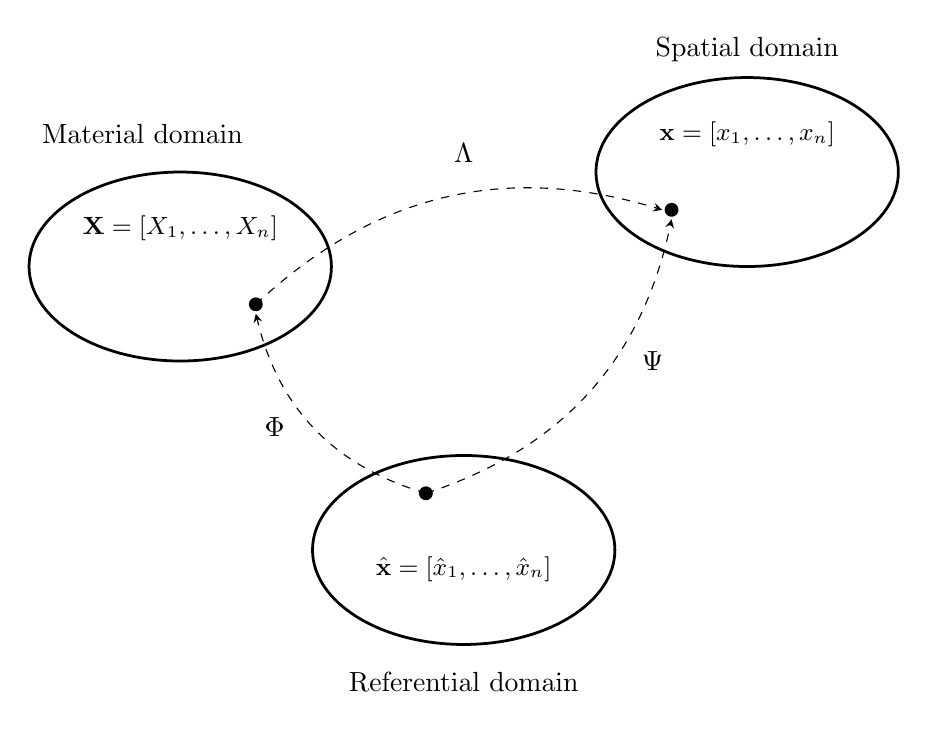
\begin{tikzpicture}[scale=2.4]
 \draw[line width=1pt] (-1.5,0) ellipse(0.8cm and 0.5cm);
 \draw[line width=1pt] (1.5,0.5) ellipse(0.8cm and 0.5cm);
 \draw[line width=1pt] (0,-1.5) ellipse(0.8cm and 0.5cm);
 
 \node[circle, fill=black, inner sep=0pt, minimum size=5pt] at (-0.2,-1.2) {};
 \node[circle, fill=black, inner sep=0pt, minimum size=5pt] at (-1.1,-0.2) {};
 \node[circle, fill=black, inner sep=0pt, minimum size=5pt] at (1.1,0.3) {};

 \node at (0.0,-1.6) {\small $\hat{\textbf{x}}=[\hat{x}_{1},\ldots,\hat{x}_{n}]$};
 \node at (-1.5,0.2) {\small $\textbf{X}=[X_{1},\ldots,X_{n}]$};
 \node at (1.5,0.7) {\small $\textbf{x}=[x_{1},\ldots,x_{n}]$};

 \draw[dashed,-stealth] (-0.2,-1.2) to[bend left=30]  (-1.10,-0.25);
 \draw[dashed,-stealth] (-0.2,-1.2) to[bend right=30] (1.10, 0.25);
 \draw[dashed,-stealth] (-1.1,-0.2) to[bend left=30]  (1.05, 0.30);

 \node at (-1.0,-0.85) {$\Phi$};
 \node at (1.0,-0.50) {$\Psi$};
 \node at (0.0,0.6) {$\Lambda$};

 \node at (-1.7,0.7) {Material domain};
 \node at (1.5,1.15) {Spatial domain};
 \node at (0.0,-2.2) {Referential domain};
\end{tikzpicture}
\end{center}
\vspace{-0.5cm}
%\source Source: The author
\label{referential domain}
\end{figure}




%\medskip
%The $\Psi$ operator maps from the referential domain
%to the spatial domain, that is, it maps the computational mesh motion
%in the spatial domain and its gradient can be represented by:
%
%\begin{equation}
%\frac{\partial \Psi}{\partial \left(\hat{\textbf{x}},t\right)} =
%\begin{bmatrix}
%\frac{\partial \textbf{x}}{\partial \hat{\textbf{x}}} & \hat{\textbf{v}}\\
%\textbf{0}^{T} & 1
%\end{bmatrix}
%\end{equation}
%
%\noindent
%where, the mesh velocity $\hat{\textbf{v}}$ and it is represented by:
%
%\begin{equation}
%\hat{\textbf{v}}_{ \left( \hat{\textbf{x}},t \right)} 
%= \frac{\partial \textbf{x}}{\partial t} \Bigg|_{\hat{\textbf{x}}}
%\end{equation}
%
%\medskip
%In addition, the $\Phi$ operator maps from the referential domain
%to the material domain, that is, it maps the computational mesh motion
%in the spatial domain and its gradient can be represented by:
%
%\begin{equation}
%\frac{\partial \Psi}{\partial \left(\hat{\textbf{x}},t\right)} =
%\begin{bmatrix}
%\frac{\partial \textbf{x}}{\partial \hat{\textbf{x}}} & \hat{\textbf{v}}\\
%\textbf{0}^{T} & \textbf{I}
%\end{bmatrix}
%\end{equation}
%
%\noindent
%where, the mesh velocity $\hat{\textbf{v}}$ and it is represented by:
%
%\begin{equation}
%\hat{\textbf{v}}_{ \left( \hat{\textbf{x}},t \right)} 
%= \frac{\partial \textbf{x}}{\partial t} \Bigg|_{\hat{\textbf{x}}}
%\end{equation}
%
%




%\medskip
%Therefore, the material point velocity that travels from 
%the material domain to the spatial domain may be obtained 
%according to the X operator:
%
%equation 4 (donea2004)
%
%\medskip
%\noindent
%Whereas, the computational mesh velocity that travels from the 
%referential domain to the spatial domain may be obtained according 
%to the Y operator:
%
%equation 7 (donea2004)
%
%\medskip
%\noindent
%Finally, we can describe the transport of any property f in 
%the spatial domain according to the ALE description as:
%
%equation 3.3 (phd2012)
